\documentclass[11pt]{article}
\usepackage{graphicx} % Required for inserting images
\usepackage{wrapfig}
\usepackage{tabularx}
\usepackage{algorithm}
\usepackage{algpseudocode}

\usepackage{subfigure}
\usepackage[a4paper,
            left=1in,
            top=1.5in,
            right=1in]{geometry}

\title{Networked software for distributed systems\\Project 5}
\date{2022-2023}

\begin{document}

\begin{titlepage}
\begin{center}
		\begin{figure}[ht]
			\centering
\includegraphics[width=0.7\textwidth]{resources/Logo_Politecnico_Milano.png}
		\end{figure}
        
        \vspace{3.5cm}

        \LARGE
        \textit{Networked software for distributed systems}\\

        \vspace{0.5cm}
        \Large
        \textbf{Analysis of COVID-19 Data}
        
        \vspace{\fill}
  
		\large
		\begin{tabularx}{\linewidth}{@{}lXl@{}}
			\textit{Authors:}  & & \textit{Professors:} \\
			Stefano Carraro      & & Prof.\@ Luca Mottola\\
			Stefano Fossati  & & Prof. Alessandro Margara \\
			Andrea Restelli & & \\
		\end{tabularx}		
		\thispagestyle{empty}

        \vspace{1cm}

        2022-2023
           
\end{center}
\end{titlepage}

\tableofcontents
\cleardoublepage

%%%
\section{Introduction}
\subsection{Request}
\subsubsection{Description}
IoT devices are used to measure environmental quantities, such as temperature and humidity, every T=10 sec.  A sliding window is applied that computes the average of the last six readings.  Should the value of the average exceed a certain threshold K, the raw readings are reported instead of the average obtained from the sliding window. The readings are reported to the backend on the regular Internet through LoRa. At the backend, information on the hottest, coolest, and most/least humid day of the month is kept in a log that is periodically communicated via email to a specific address. The log must be persistent, that is, rebooting the backend should not make the backend system lose the data gathered until that time.
\subsubsection{Assumption and Guidelines}
The backend may be assumed to have sufficient memory, in both RAM and persistent storage, to handle the application load.
\subsubsection{Technologies}
\begin{itemize}
    \item Node-Red
    \item Contiki-NG or mBad
\end{itemize}

\subsection{Additional Assumptions}
\begin{itemize}
    \item The sensor has a precise global time 
    \item The sensor data are randomly generated from an integer range
    \item The coldest/hottest and most/less humid day refer to the day of the month with the lowest/highest average value calculated from all data measured in a day
\end{itemize}
\cleardoublepage

%%%


\section{Design}
The problem description specifies two main components of the system:
\begin{itemize}
    \item The IoT sensors;
    \item The backend;
\end{itemize}

The specification requires the backend to be persistent. So we decided to use a database in order to satisfy the requirement saving the data persistently.

\begin{wrapfigure}{l}{0.5\textwidth}
    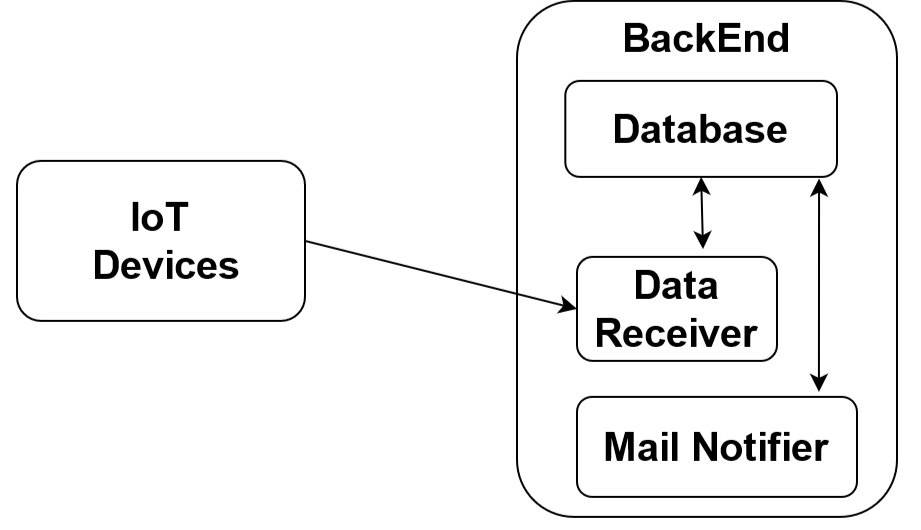
\includegraphics[width=0.8\linewidth]{resources/Design.png} 
    \caption{The high-level structure of the system}
\end{wrapfigure}

The IoT sensors measure data that are partially elaborated on the sensor itself and after that they send the data collected to the backend through a network connection. The data receiver component of the backend receives the information, modifies them and saves them in the database. \\
The other component of the backend, the mail notifier, at every first day of every month retrieves the data of the previous month from the database. Then, firstly the data is elaborated to calculate the average temperature and humidity for each day of the previous month. Secondly, the hottest, coolest, and most/least humid days of that month are determined. Finally this information is sent to a specific email address.

\subsection{Focus on Sensor Architecture}


The sensor communication is made through a RLP protocol. This protocol enables the sensors to create a tree shape routing. Each sensor needs to locate another sensor within its radio range that is connected to the root of the tree. In our scenario the root is exposed to the external network and is connected to the MQTT broker.
In our sensor communication setup, the sensors send messages to the root tree. This is because the sensors need to transmit their messages to the backend, and therefore, they only need to address the received messages from the sending sensor to the root tree. 
\begin{figure}[H]
    \centering
    \subfigure[Sensor Routing Path]{
        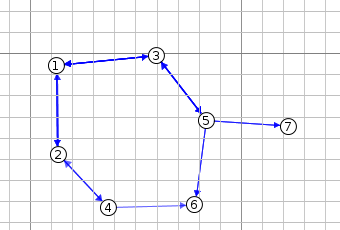
\includegraphics[width=6cm]{resources/Sensor_Routing.png}
        \label{fig:navigation_evaluations}
    }
    \subfigure[Sensor 5 Distance Range]{
        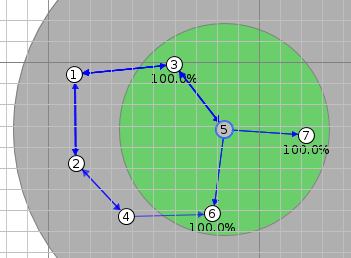
\includegraphics[width=6cm]{resources/Sensors_Distance_Range.png}
        \label{fig:presentation_evaluations}
    }
    \caption{RPL Routing: Node 1 is the root connected to the external network, Node 2,3,4 are the temperature sensors, 5,6,7 are the humidity sensors}
\end{figure}

\section{Implementation and Deployment}
\subsection{Technologies}
\begin{itemize}
    \item IoT: \\
    Contiki-NG is the operating system used for the IoT devices programming. This is a technology requirement and also the IoT technology that has been presented in this course.
    \item Backend logic: \\
    The logical part of the backend is implemented using Node-red.
    \item Backend database: \\
    We have decided to use a database in order to persistently store the data. We have chosen a no-SQL DB in particular MongoDB. We have opted for MongoDB because it uses collections to save data. In our case this feature is very useful because we can insert the data, after a few type field adjustments, in different collections that correspond to the different type of data that the sensors have measured.
    \item Network communication: \\
    During the course we saw the implementation of MQTT protocol with Contiki-NG. This protocol is widely used in the IoT and also is very convenient in our project because it allows us to publish on different topics the different readings type of the sensor (in our case humidity and temperature).
\end{itemize}
\begin{figure}[h]
    \centering
    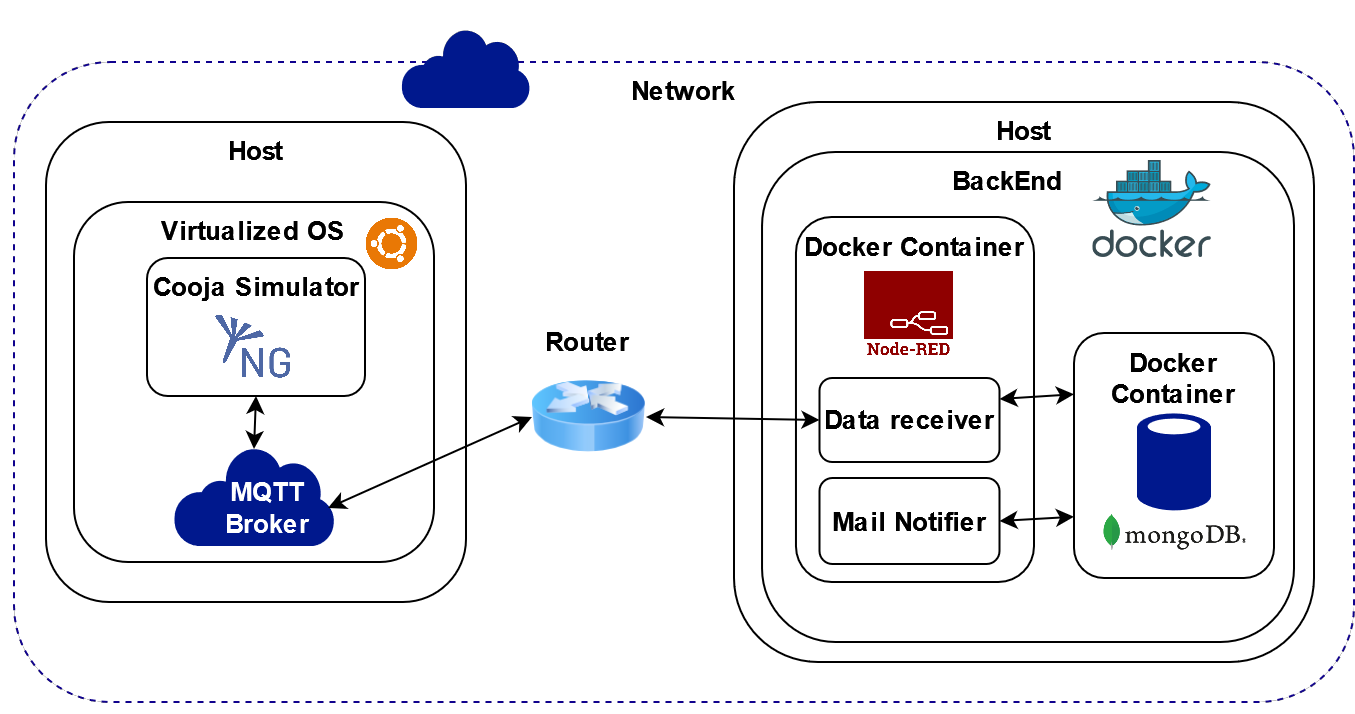
\includegraphics[width=15cm]{resources/Technologies.png}
    \caption{The high-level structure of the system with the technologies}
\end{figure}

\subsection{Implementation}
\subsubsection{IoT }
The data taken by the sensor are simulated through a random generator between a range of values. After that the data is taken, the sensors execute a sliding window algorithm as specified by the requirements.
\begin{algorithm}
    \caption{Sliding Window Algorithm}\label{alg:cap}
    \begin{algorithmic}
        \If{Start}
            \State Array=[0,0,0,0,0,0]
            \For{$(i=0, i<Array.length, i++)$}
                \State Array[i] = GenerateValue();
            \EndFor
        \ElsIf{}
            \State var newValue = GenerateValue();
            \For{$(i=1, i<Array.length, i++)$}
                \State Array[i] = Array[i-1];
            \EndFor 
            \State Array[0] = newValue;
        \EndIf
    \end{algorithmic}
\end{algorithm}

This algorithm is run periodically by each sensor. In particular the GenerateValue() function returns a random value in a value range specified in the sensor configuration. It is used for emulating the temperature/humidity readings.
After that the sensor has generated a new value and has put it in the sliding window array, the sensor checks that the average of the values in the array is lower or higher than the threshold configured in the sensor configuration file.
If it is lower, the sensor sends the value average of the array, instead it sends the whole array.

\subsubsection{Backend}
The backend is divided into two main flows:
\begin{itemize}
    \item In the first flow, the backend listens to the MQTT topic where the sensors publish the data. When new data is received, it is saved in the database after undergoing specific data transformations.
    \item The second flow checks if it is the first day of the month. If it is, the system queries the database to retrieve all the data from the previous month. The backend then computes the coldest/hottest and most/least humid days by considering the average of the data recorded within a single day.
\end{itemize}
\subsection{Deployment}
\subsubsection{IoT devices}

The IoT devices are emulated by Cooja. It allows us to create IoT devices, so in our case humidity and temperature sensors, and to position them in a virtual area.
Cooja runs on a Ubuntu Virtual Machine (the one provided by the professor) that also hosts an MQTT broker. So Cooja connects the sensors to the MQTT broker. 
\begin{figure}[H]
    \centering
    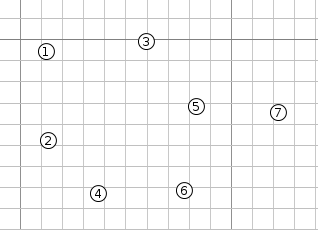
\includegraphics[width=6cm]{resources/Sensors_Position.png} 
    \caption{The position of the sensor. 
    Node 1 is the root connected to the external network, Node 2,3,4 are the temperature sensors, 5,6,7 are the humidity sensors}
\end{figure}
\subsubsection{BackEnd}
The backend is hosted on Docker, utilizing separate containers for Node-RED and MongoDB. Node-RED is contained within its dedicated container, while MongoDB resides in another Docker container, which exposes the connection for integration with Node-RED. Node-RED is connected to an MQTT broker, allowing for communication and data exchange between the MQTT broker and the backend system.

\subsubsection{Whole System}
The two parts of the system are hosted on different physical devices that are connected under the same network.

\end{document}
